\documentclass{IEEEtran}

\usepackage{cite}
\usepackage{amsmath}
\usepackage{amssymb}
\usepackage{url}
\usepackage{graphicx}
\usepackage{booktabs}
\usepackage{microtype}
\usepackage[table]{xcolor}
\usepackage{tikz}
\usetikzlibrary{positioning,arrows.meta,fit,backgrounds}
\usepackage[hidelinks]{hyperref}

% Phase color palette
\definecolor{phase1blue}{RGB}{52,152,219}      % Environment / Input
\definecolor{phase2green}{RGB}{46,204,113}     % Context Observation
\definecolor{phase3orange}{RGB}{230,126,34}    % Routing Decision
\definecolor{phase4purple}{RGB}{155,89,182}    % Evaluation / Feedback

\title{Fairness-Aware Routing in Quantum Networks and Clinical Settings\\[0.3em]
{\large\textit{via Multi-Armed, Contextual, and Informative Bandit Methods}}\\[0.3em]
{\large\textit{(Approach Writeup)}}}

\author{%
\begin{minipage}{0.48\textwidth}
\begin{center}
{\bf Piter Z. Garcia}\\
\begin{small}
MS Data Science / Decision-Making \& Algorithmic Fairness\\
Rochester Institute of Technology (RIT)\\
{\it pizg8794@g.rit.edu}
\end{small}
\end{center}
\end{minipage}
\hfill
\begin{minipage}{0.48\textwidth}
\begin{center}
{\bf Dr. Daniel Krutz, Travis Desell}\\
\begin{small}
Department of Software Engineering, Data Science\\
RIT Research Advisors\\
{\it dxkvse@g.rit.edu, tjdvse@g.rit.edu}
\end{small}
\end{center}
\end{minipage}%
}

\begin{document}
\maketitle

%% ─────────────────────────────────────────────────────────────
\section{Approach Overview}
%% ─────────────────────────────────────────────────────────────

This work is grounded in a single unifying observation: both quantum-network
routing and clinical resource allocation are, at their core, \textit{routing
problems}. In quantum networking, entanglement and qubit resources must be
routed across competing paths and flows under probabilistic link success and
scarcity. In clinical settings, diagnostic and treatment resources---tests,
follow-ups, escalation decisions---must be routed among patients under
uncertainty, partial context, and operational constraints. In both cases,
\textit{unfair routing is not merely an equity problem; it is a performance
problem.} When one group of flows or patients is systematically
deprioritized, the downstream degradation in success probability, latency,
or care quality is direct and measurable. This shared structure makes the
two domains analytically equivalent and motivates a unified evaluation
framework.

The methodological contribution is a shared, reproducible bandit-method
evaluation framework spanning three levels of context richness:
non-contextual multi-armed bandits (MABs), contextual multi-armed bandits
(CMABs), and informative contextual multi-armed bandits (iCMABs). The
framework applies the same interaction model, fairness-logging pipeline, and
comparison logic in both settings so that findings in one domain directly
inform the other.

Two prior works anchor the testbeds. Equitable bioinformatics work provides
the clinical fairness foundation and subgroup disparity metrics
\cite{garcia2025equitable_bioinformatics}, while threat-aware quantum
routing work provides the domain-realistic network routing and
resource-allocation environment \cite{garcia2026threat_aware_quantum_routing}.
The cross-domain design is a deliberate research choice: quantum networking
represents an emerging frontier technology with proven potential to transform
communication, computation, and resource allocation. Pairing it with a
clinical setting that has immediate human impact---and sharing routing as the
structural bridge---positions this work at the intersection of present
necessity and future breakthrough.

%% ─────────────────────────────────────────────────────────────
\section{Motivating Workflows}
%% ─────────────────────────────────────────────────────────────

Two concrete routing workflows ground the shared domain model in
domain-specific operational constraints.

\subsection{Clinical Routing Workflow}
In the clinical setting, the decision-maker repeatedly routes resources:
ordering an initial screen, selecting a confirmatory test, or escalating
follow-up when a prior result is ambiguous. Each of these is a routing
decision that determines which patient receives which diagnostic or
therapeutic resource at which time. Routing context---patient features,
prior outcomes, sample quality indicators---may be incomplete, delayed, or
noisier for some demographic groups. When context quality is uneven, the
routing policy may systematically under-resource certain subgroups,
producing higher false-negative rates, delayed escalation, or inferior
downstream care. Clinical fairness is therefore treated as a time-evolving
property of the routing process rather than a static post-hoc audit.

\subsection{Quantum Routing Workflow}
In the quantum-network setting, the decision-maker routes entanglement:
selecting paths and allocating scarce entanglement-generation attempts among
competing flows under probabilistic link success and changing network
conditions. Routing context---link-quality estimates, queue and load signals,
or threat indicators---can be noisy, stale, or only partially observed. When
context is unreliable, routing policies may consistently assign degraded
paths or insufficient resources to certain flow groups, creating
service-equity gaps in success probability, latency, and resource access.
This interpretation makes quantum routing a genuine fairness domain rather
than a purely performance-oriented benchmark.

%% ─────────────────────────────────────────────────────────────
\section{Shared Domain Model}
%% ─────────────────────────────────────────────────────────────

The shared domain model makes the common routing-decision structure explicit
across both testbeds while preserving domain-specific interpretations of
states, actions, rewards, and fairness metrics. The model is organized into
four phases, each color-coded in Figure~\ref{fig:domain_model}:
(1)~\textcolor{phase1blue}{\textbf{Environment / Input}} (blue),
(2)~\textcolor{phase2green}{\textbf{Context Observation}} (green),
(3)~\textcolor{phase3orange}{\textbf{Routing Decision}} (orange), and
(4)~\textcolor{phase4purple}{\textbf{Evaluation and Mitigation}} (purple).

The four-phase structure is identical in both domains. What differs is the
operational semantics: in the clinical domain, a routing action is a
diagnostic or treatment decision; in the quantum domain, it is a path
selection or entanglement-allocation decision. Fairness in both cases is
measured as a disparity in outcomes across subgroups---patient demographics
in the clinical setting, flow or user groups in the quantum setting.

%% ─────────────────────────────────────────────────────────────
\section{Design Rationale and Novelty}
%% ─────────────────────────────────────────────────────────────

\subsection{Q1: Why do it this way, and why has it not been done before?}
No prior work evaluates fairness-aware sequential routing under a unified
bandit framework spanning both clinical resource allocation and quantum
network entanglement routing. Existing literature treats these domains in
isolation: contextual bandits for clinical trials focus on treatment
optimization without modeling routing fairness across patient subgroups;
quantum routing research optimizes throughput and fidelity without examining
service-equity disparities under partial and noisy context. The critical gap
is the recognition that routing unfairness and routing performance are
inseparable in both domains---a connection no existing approach has
formalized or evaluated.

Quantum networking is not a distant hypothetical. It is a proven, emerging
technology with documented potential to reshape communication, computation,
and resource distribution. Pairing it with a clinical domain that directly
affects human health and equity is not an arbitrary coupling. It is a
deliberate positioning of this research at the frontier where technological
advancement and human fairness intersect. Studying both together produces
findings that can simultaneously improve today's clinical routing systems
and inform the design of fair routing mechanisms in tomorrow's
quantum-enabled infrastructures.

\subsection{Q2: Why is this approach better than others?}
Single-domain approaches cannot test whether a fairness principle is
structurally general or merely domain-specific. A study limited to clinical
bandits or to quantum routing alone provides no evidence that the findings
transfer or that the framework is robust across different state spaces,
reward structures, and fairness definitions. By applying the same interaction
model and logging pipeline across two structurally analogous but operationally
different routing domains, this approach produces findings that are
simultaneously more credible and more generalizable than any single-domain
alternative.

Approaches that apply fairness as a post-hoc audit cannot capture how
routing decisions compound over time or how disparities evolve under
learning. This framework measures fairness at every step of the decision
process, making it possible to detect early-onset disparities, evaluate
mitigation mechanisms in real time, and compare policies under the same
partial-feedback conditions that make routing decisions difficult in practice.

\subsection{Q3: What design and implementation decisions were made, and why?}
\textit{Bandit methods over full reinforcement learning.} The bandit
formulation is chosen because both routing domains involve partial feedback:
the decision-maker observes only the outcome of the chosen route, not
counterfactual outcomes of unchosen alternatives. Full RL would require
richer state-transition modeling that is neither available nor necessary to
answer the fairness questions posed.

\textit{Simulation-first clinical testbed.} A simulation environment is used
intentionally so that missingness, noise, and group-specific context
degradation can be introduced under controlled, reproducible conditions
without dependence on sensitive patient data. This is not a limitation; it
is the correct design for isolating the effect of routing-context quality on
fairness outcomes.

\textit{Extension of existing quantum routing environment.} Rather than
constructing a new quantum testbed, the approach extends an already-grounded,
threat-aware quantum routing environment
\cite{garcia2026threat_aware_quantum_routing}. This preserves domain
realism, avoids the credibility risk of a fabricated testbed, and ensures
quantum routing findings reflect conditions studied in prior work.

\textit{Three-level context spectrum (MAB, CMAB, iCMAB).} The spectrum
directly operationalizes the core research question: whether routing fairness
can be improved through richer context, or whether context itself---when
unevenly available---amplifies rather than reduces disparities. The three
levels create a controlled ladder of information richness that isolates the
effect of context quality on routing equity.

\subsection{Q4: How do these decisions connect to the domain model?}
Every design decision maps directly to a specific phase in the shared domain
model (Figure~\ref{fig:domain_model}). The choice of bandit methods over
full RL is a \textbf{Phase~3} decision: it constrains the policy family to
methods that operate under partial feedback, which is the feedback structure
defined in \textbf{Phase~4}. The simulation-first clinical design and the
quantum environment extension are \textbf{Phase~1} decisions: they determine
what enters the testbed and under what conditions. The three-level context
spectrum is a \textbf{Phase~2} decision: it controls what routing context is
observable and how degraded it can be. The shared fairness-logging and
mitigation loop is a \textbf{Phase~4} decision: it ensures fairness is a
per-step, first-class output. The domain model is therefore not a diagram
added after the fact; it is the organizational structure that determined
each design choice.

%% ─────────────────────────────────────────────────────────────
\section{Implementation and Evaluation Plan}
%% ─────────────────────────────────────────────────────────────

The implementation plan prioritizes reproducibility and systematic fairness
evaluation across both testbeds. The clinical simulation models sequential
routing decisions---test ordering, retesting, and escalation---under
conditions where some patient groups have weaker or noisier observed context.
The quantum routing environment represents path selection and
entanglement-resource allocation under probabilistic link success, changing
load, and limited quantum resources. Both testbeds expose the same policy
interface so that MAB, CMAB, and iCMAB methods are evaluated under a shared
logging and analysis pipeline.

The reward layer tracks utility-oriented routing outcomes: accuracy, cost,
success rate, and latency. The fairness layer tracks domain-specific routing
disparities: clinical false-negative and delayed-escalation gaps across
patient subgroups; quantum service-equity gaps in routing success or latency
across flow groups. Fairness is therefore a first-class output at every step.

Experiments run from explicit configuration files with fixed random seeds and
per-step metric logging. At least one fairness-aware mitigation mechanism is
evaluated inside the same framework so that the final comparison includes
both baseline disparity assessment and the effect of active mitigation under
learning.

%% ─────────────────────────────────────────────────────────────
\section{Research Contribution}
%% ─────────────────────────────────────────────────────────────

This work makes three distinct contributions. First, it identifies routing
as the structural common ground between clinical resource allocation and
quantum network entanglement distribution, and builds the first
fairness-aware sequential decision framework that evaluates both under
identical experimental conditions.

Second, it provides the first systematic comparison of non-contextual,
contextual, and informative-context bandit policies with respect to routing
fairness, making it possible to determine whether richer context reduces
routing disparities or introduces new ones when context quality is uneven
across groups.

Third, it advances a new direction in applied fairness research by connecting
a domain with immediate human health impact---clinical routing---to an
emerging breakthrough technology---quantum networking---through a shared
structural property. This positions the findings not only as an evaluation
of current systems, but as a foundation for designing fairer routing
mechanisms in next-generation quantum-enabled infrastructures.

%% ─── Figure placed at end to preserve two-page layout ───────
\begin{figure*}[!b]
\centering
\resizebox{0.97\textwidth}{!}{%
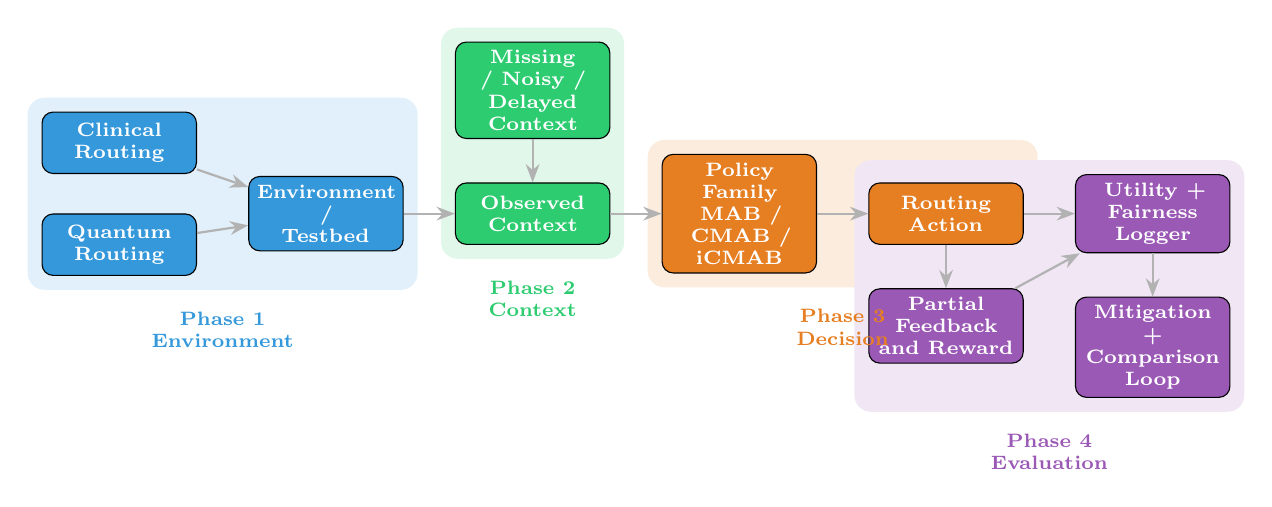
\begin{tikzpicture}[
  font=\scriptsize,
  box/.style={draw, rounded corners=4pt, align=center,
              text width=1.75cm, minimum height=0.78cm,
              inner sep=3pt, text=white, font=\scriptsize\bfseries},
  phase1/.style={box, fill=phase1blue},
  phase2/.style={box, fill=phase2green},
  phase3/.style={box, fill=phase3orange},
  phase4/.style={box, fill=phase4purple},
  arr/.style={-Stealth, thick, gray!60},
  lbl/.style={font=\scriptsize\bfseries, align=center}
]

%% Phase 1 — Environment / Input (blue)
\node[phase1] (clin)  {Clinical\\Routing};
\node[phase1, below=0.5cm of clin]  (quant) {Quantum\\Routing};
\node[phase1, right=0.65cm of clin, yshift=-0.9cm] (env) {Environment /\\Testbed};

%% Phase 2 — Context Observation (green)
\node[phase2, right=0.65cm of env]  (ctx) {Observed\\Context};
\node[phase2, above=0.55cm of ctx]  (deg) {Missing / Noisy /\\Delayed Context};

%% Phase 3 — Routing Decision (orange)
\node[phase3, right=0.65cm of ctx]  (pol) {Policy Family\\MAB / CMAB / iCMAB};
\node[phase3, right=0.65cm of pol]  (act) {Routing\\Action};

%% Phase 4 — Evaluation / Feedback (purple)
\node[phase4, below=0.55cm of act]  (fb)  {Partial Feedback\\and Reward};
\node[phase4, right=0.65cm of act]  (log) {Utility + Fairness\\Logger};
\node[phase4, below=0.55cm of log]  (mit) {Mitigation +\\Comparison Loop};

%% Arrows
\draw[arr] (clin)  -- (env);
\draw[arr] (quant) -- (env);
\draw[arr] (env)   -- (ctx);
\draw[arr] (deg)   -- (ctx);
\draw[arr] (ctx)   -- (pol);
\draw[arr] (pol)   -- (act);
\draw[arr] (act)   -- (fb);
\draw[arr] (act)   -- (log);
\draw[arr] (fb)    -- (log);
\draw[arr] (log)   -- (mit);

%% Colored phase background bands
\begin{pgfonlayer}{background}
  \node[fill=phase1blue!15, rounded corners=6pt, inner sep=5pt,
        fit=(clin)(quant)(env)] (bg1) {};
  \node[fill=phase2green!15, rounded corners=6pt, inner sep=5pt,
        fit=(ctx)(deg)] (bg2) {};
  \node[fill=phase3orange!15, rounded corners=6pt, inner sep=5pt,
        fit=(pol)(act)] (bg3) {};
  \node[fill=phase4purple!15, rounded corners=6pt, inner sep=5pt,
        fit=(fb)(log)(mit)] (bg4) {};
\end{pgfonlayer}

%% Phase labels
\node[lbl, text=phase1blue,   below=0.15cm of bg1] {\textbf{Phase 1}\\Environment};
\node[lbl, text=phase2green,  below=0.15cm of bg2] {\textbf{Phase 2}\\Context};
\node[lbl, text=phase3orange, below=0.15cm of bg3] {\textbf{Phase 3}\\Decision};
\node[lbl, text=phase4purple, below=0.15cm of bg4] {\textbf{Phase 4}\\Evaluation};

\end{tikzpicture}%
}
\caption{%
  Shared domain model across both testbeds, organized into four color-coded
  phases.
  \textcolor{phase1blue}{\textbf{Phase 1 (blue) --- Environment / Input:}}
    The clinical routing workflow and the quantum routing workflow feed into a
    shared testbed interface.
  \textcolor{phase2green}{\textbf{Phase 2 (green) --- Context Observation:}}
    The system observes available routing context, subject to missingness,
    noise, or delay---treated as an explicit part of the research question.
  \textcolor{phase3orange}{\textbf{Phase 3 (orange) --- Routing Decision:}}
    A policy from the selected method family (MAB, CMAB, or iCMAB) selects a
    routing action under the observed context.
  \textcolor{phase4purple}{\textbf{Phase 4 (purple) --- Evaluation and
    Mitigation:}}
    The environment returns partial feedback; utility and fairness metrics
    are logged per step; and baseline and fairness-aware mitigation policies
    are compared within the same loop.}
\label{fig:domain_model}
\end{figure*}

\begin{thebibliography}{9}\setlength{\itemsep}{0em}
\bibitem{garcia2025equitable_bioinformatics}
Garcia, P. Z. Equitable Bioinformatics: Enhancing Diagnostic
Decision-Making through {RNA} and Biomarker Data. Course paper
(ISTE~780 Phase~4), Rochester Institute of Technology, 2025.
\bibitem{garcia2026threat_aware_quantum_routing}
Garcia, P. Z. Threat-Aware Evaluation of Quantum Entanglement Routing
and Qubit Allocation via Hybrid Contextual Bandits. Unpublished
manuscript (GA-Work internal draft), Rochester Institute of Technology,
2026.
\end{thebibliography}

\end{document}
